\documentclass[12pt]{article}

\title{Using idiolects to improve word prediction}
\author{Wessel Stoop}

\usepackage{covington}
\usepackage{graphicx}
\usepackage{float}
\usepackage{apacite}
\usepackage{qtree}

\renewcommand{\familydefault}{\sfdefault}

\let\stdsection\section
\renewcommand\section{\newpage\stdsection}

\begin{document}

\begin{table}[b]
\begin{tabular}{ll}
\textbf{Master's thesis}&\\
Name&Wessel Stoop\\
Student numbers&s0808709 (Nijmegen), u1249664 (Tilburg)\\
Supervisor&Antal van den Bosch\\
Period&Spring 2013\\
\end{tabular}
\end{table}

\maketitle

\begin{figure}
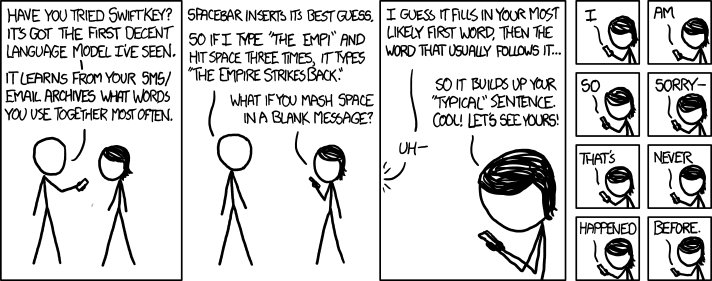
\includegraphics[scale=0.5]{swiftkey}
\end{figure}

\clearpage

\tableofcontents

\section{Summary/samenvatting}

\subsection{English}

\subsection{Nederlands}

\section{Introduction}

\subsection{Word prediction}

%Eerst algemeen
%Daarna laatste ontdekkingen

\subsection{Idiolects}




%Uitleg: twee delen. Dat zijn de volgende twee sections






\section{The algorithm: Soothsayer}

\subsection{Introduction}

\subsubsection{Soothsayer}
The goal of this chapter is to build the best word prediction algorithm possible, from the ground up. We will start with a very basic application that uses word uniqueness thresholds to predict the word the user is keying in, and add more components and smaller improvements step by step. I have given the resulting system the working title \emph{Soothsayer}, for ease of reference.

An important thing to note is that Soothsayer works with independent modules. A module can be seen as a function that takes some input (for example, the letters of the word the user is currently keying in) and uses a language model to generate:

\begin{enumerate}
\item The most likely prediction
\item The second most likely prediction
\item The third most likely prediction
\item In case of a context-sensitive module, how many other predictions the model provided
\end{enumerate}

Modules can be either context-insensitive or context-sensitive, as will be explained in much detail in section \ref{ci} and section \ref{cs} respectively, and use one language model. In a set-up with two language models (which is the main set-up used in chapter \ref{model}), we thus have four possible modules:

\begin{enumerate}
\item Model 1, context-sensitive
\item Model 1, context-insensitive
\item Model 2, context-sensitive
\item Model 2, context-insensitive
\end{enumerate}

Modules can be concatenated in such a way that a second module takes over once the first modules no longer has predictions, a third module takes over once the second one no longer has predictions, etcetera. This makes it possible to use multiple prediction techniques \emph{and} multiple language models in one prediction system.

\subsubsection{Evaluation}
In this chapter, I will propose an addition to Soothsayer and then measure to what extent it improves the number of keystrokes saved several times. But how does one measure how many keystrokes are saved exactly? In other words, what is the best way to evaluate a word prediction system?

One possibility is to provide the user with a list of the $n$ most likely predictions \cite{Lesher+99,Fazly+03}. This approach has the advantage that it results in high percentages of keystrokes saved (in particular when $n$ is set to a high value, because this means the system can do multiple guesses at once, while only one has to be correct), but also has downsides. As \citeA{vandenbosch11} notes: 

\begin{quotation}
[I]n many devices and circumstances it is inefficient or impossible to present [...] suggestion lists. Inspecting a list of suggestions also poses a larger cognitive load than checking a single suggestion, and furthermore it is unclear how scrolling, browsing and selecting items from this list should be counted in terms of keystrokes.
\end{quotation}

For this reason, I will follow \citeA{vandenbosch11} and always calculate the number of keystrokes that could have been saved when the user was presented only one prediction at a time. Predictions can be accepted with the space key. Because this is sometimes problematic (for instance, if the user wanted to type \emph{sun}, but Soothsayer predicts \emph{sunday}, hitting space would lead to the wrong word), a rejection is also calculated as a keystroke. The number of keystrokes that can be saved if the autocompletion application works this way will be called \textbf{Classical Keystrokes Saved} (CKS) in the remainder of this thesis.

On the other hand, current popular smartphone applications suggest this approach might be too strict. The popular smartphone application SwiftKey\footnote{\url{http://www.swiftkey.net/}} always shows the user three predictions, which seem to be (1) what the user has keyed in so far, (2) the most likely prediction and (3) the second most likely prediction. In case the user has not yet started typing the next word, option (1) is replaced by the third most likely prediction. Because smartphones use a touchscreen as an input device, no extra keystrokes are needed. The percentage of keystrokes that can be saved when two (and sometimes three) predictions were shown will be referred to as \textbf{SwiftKey Keystrokes Saved} (SKKS).

A thing to notice is that both measures reflect the percentage of keystrokes saved in an ideal situation; that is, when the user accepts a correct prediction immediately once it is available. As will be discussed further in section \ref{early}, this is not necessarily the case. 

%referenties nalezen, meer toevoegen
%wordt dat echt discussed? NEE
%Hit ratio. Time-saving, person saving.

\subsubsection{What Soothsayer is not}
There are many possible approaches to take when building an autocompletion system. Because it would take too much time to try all of these approaches (and all combinations of them), I had to set limitations. Therefore, before I explain and defend the workings of Soothsayer, I therefore would like to list the most importat decisions, so the reader has a rough idea of what is coming. 

\begin{itemize}
\item \textbf{Soothsayer does not predict more than one word at a time}. Some scholars have investigated the possibility to predict multiple words at the same time [[refs]]. This can very fruitful: if a word prediction system knows that \emph{on the b} should be \emph{on the basis of} it makes more sense to offer this as a whole, instead of first asking whether \emph{basis} is correct. However, multiword prediction comes with a lot of downsides: every extra word that is predicted doubles the chance of making an incorrect prediction, it is unclear what a user should do if he/she accepts the first word, but the not the second word (or vice versa), and how this should be counted in terms of keystrokes, and giving multiple words forces the user to plan ahead a few words while typing, which might not be how the user prefers to write. %kijken wat antal zegt

\item \textbf{Soothsayer does not focus on one specific domain of word prediction, but works for word prediction is general}. Niet Google.

\item \textbf{Soothsayer is not designed for mobile phones, but can be integrated into any kind of software, on any device}. When discussing this subject with others, I noted that word prediction is often confused with T9. T9 is a system in which every number corresponds with 3 or 4 characters (\emph{1} = \emph{.,!}, \emph{2} = \emph{abc}, \emph{3} = \emph{def}, etc.). A T9 system allows the users to press all numbers only once, and tries to figure out which word the writer probably intended; for example, \emph{233} can correspond to \emph{bed}. Although there is some language technology involved in systems like these (the system should know enough about language to figure out \emph{aef}, \emph{cfe} \emph{bde}, etc. or not words), this is not what Soothsayer does; Soothsayer does try to guess what the user wanted to say \emph{after} the user keyed it in, but \emph{before}. 

Besides that, Soothsayer is designed to be indepent of device of input method. Instead, it includes a \emph{server mode} and an \emph{HTTP-server mode}, making it very easy to integrate into any piece of software. This means it is very well possible that Soothsayer will be used together with a T9-system one day.

\item \textbf{Soothsayer does not use hand-made, language-specific rules, but is fully language independent}. In the early of Natural Language Processing, many scholars have tried to build NLP systems by including as much as linguistic knowledge of possible. In terms of a word prediction system, this could for example entail including a system that recognizes personal pronouns, and only provides verbs that agree with these pronouns, or making sure that after the neutral article \emph{het} only neuter words were suggested. 

Soothsayer does not work this way. Instead, it is given as much training material as possible, and tries to learn from that. So Soothsayer might know the noun \emph{kast} probably does not follow the article \emph{het}, but because it has not encountered that during training, not because I told it so. As a result of this, Soothsayer is fully language independent: if it is trained on Dutch data, is will predict Dutch words, if it is trained on Swahili, it will predict Swahili words. In fact, the context-sensitive modules will often give correct predictions even with mixed training data.

\end{itemize}

\subsection{Context-insensitive modules} \label{ci}

Context-insensitive modules only use information of the word the user is currently keying in. In sentence \ref{only_c}, for example, only the c will be used for prediction. 

\begin{examples}
\item I ate too much c \label{only_c}
\end{examples}

This means that a prediction like \emph{communication} is fully possible, despite the context, just because \emph{communication} starts with a c. This also means that at the beginning of a each new word no prediction will be available, because the module has no material to work with.

Despite these limitations, context-insensitive modules can already save a lot of keystrokes, because the first few letters of a word impose enormous limitations on what letters can possibly follow.

\begin{examples}
\item This is good communic \label{communic}
\end{examples}

In sentence \ref{communic}, we already know from \emph{communic} that \emph{ation} or \emph{ative} will follow, simply because these are the only two words that start with \emph{communic}. The first iteration of the context-insensitive module I will propose will be based on this idea: at a certain point in a word, other words are no longer an option. This point is called the \emph{uniqueness threshold}.

\subsubsection{First iteration: using uniqueness thresholds}

The first iteration of the context-insensitive module will take the word the user is currently keying in as the input. If, on the basis of what has been given, only one word is still possible, this word will be returned as a prediction. To know which words are 'possible', the module uses a lexicon. An important characteristic of this approach is that is does not or rarely make mistakes (assuming a large enough lexicon): only words the system is 100\% sure about are predicted.

To test this, I exported all emails I have sent between February 2009 and February 2013, containing [[x]] words. I formed a lexicon on the basis of the first 90\% of the material, and tested on the remaining 10\% - the most recent emails. The testing was done by simulating a user keying in the material letter by letter. Once the correct prediction was available, the remaining letters of that word were skipped. The percentages were calculated by dividing the amount of skipped letters by the total amount of letters.

This resulted in a \textbf{CKS of 5\%} and an \textbf{SKKS of 5\%}. These are relatively low percentages, but that can be explained by the fact that many of the words are too short to reach their uniqueness thresholds. For example, the word \emph{the} will never be predicted because even when the word is finished, alternatives are still possible (\emph{these}, \emph{there}, etc.).

\subsubsection{Second iteration: using word frequencies}
A solution to the fact that short words never reach their uniqueness threshold can be to give the prediction \emph{before} the word has reached its recency threshold. This can lead to situations where the correct word is predicted long before the uniqueness threshold is reached, which increases the number of keystrokes saved. However, this also means many incorrect predictions will be given; we sacrifice the accuracy of the system. To what extent this is a problem is unclear: at the one hand, the user is forced to accept and reject more predictions while typing, which probably increases the cognitive load, at the other hand all the user has to do to reject a prediction is to continue typing; no extra actions are needed. A systematic investigation of the extra cognitive load during typing while using a word prediction system is beyond the scope of this thesis; because no extra actions are needed to reject the prediction it will be assumed the saved keystrokes are worth the extra cognitive load.

If a prediction is given when multiple words are still a possibility, a system that picks the word with the highest chance of occurring will of course have the best results. These chances are reflected by the frequency of the words in the language. Therefore, each time the users keys in a new letter, Soothsayer will go through a frequency list. The first (and thus most frequent and most likely) word that matches with what has been keyed in so far will be given as a prediction.

To test this, the email corpus from the previous section was used. The simulation showed a much higher percentage of keystrokes can be saved this way: a \textbf{CKS of 20 \%} and an \textbf{SKKS of 27 \%}. For this reason, this second iteration of the algorithm is the algorithm that will be used when referring to the 'context-insensitive' module in the remainder of this thesis.

\subsection{Context-sensitive modules} \label{cs}

Context-sensitive modules make use of the words that came before the current word to limit what words are predicted. For sentence \ref{only_c}, repeated here as \ref{only_c_r}, the context would be the words \emph{ate}, \emph{too} and \emph{much}.

\begin{examples}
\item I ate too much c \label{only_c_r}
\end{examples}

This context is compared with a training corpus, which results in a list of words which often occur together with the words from the context. This approach probably returns words like \emph{cookies} or \emph{cake} (because of the word \emph{ate}), while the word \emph{communication} is no longer an option because it probably did not occur in this context in the training texts.

\subsubsection{Word prediction as a classification task}

To make use of the context, Soothsayer approaches word prediction as a classification task. Classification means finding a \emph{class} for an \emph{instance} on the basis of its \emph{features}. For instance, you could say a person (instance) is a man (class) because he has a beard, a low voice, short hair and is tall (features). In some cases, classification is simple: when sorting garbage, you use only 1 feature (material) which results in the correct class (paper, glass, plastic, biodegradable, miscellaneous) 100\% of the time, but in most cases it is not; for instance, for a person with a beard you can be pretty sure it is a man, but not all men have beards. And for the other features, there also are women with low voices, women with short hair and women who are tall. In cases like this, it is the combination of features that (in most cases) will result in the correct class.

For word prediction, we use the context as instance, the words in the context as features, and the word which follows this context as class. This means that instead of only two classes (as in the gender example), we have a separate class for every word that could possibly be predicted. Thus, if we want to predict that \emph{cookies} follows the context \emph{ate too much}, we hope that classifying the instance \emph{ate too much} on the basis of its features (the words \emph{ate}, \emph{too} or \emph{much}) will result in the correct class label \emph{cookies}.

\subsubsection{Nearest neighbour classification}

There are many algorithms to do classification automatically. Soothsayer uses the $k$-nearest neighbour classification method. $k$-nearest neighbour classification (henceforth \emph{KNN}) means that the class is determined on the basis of similar cases in a training corpus. How many cases are taken into consideration, $k$, can be determined beforehand. For example, let us set $k$ to 1 and take the following instances as a training corpus:

\begin{examples}
\item one two three (four)
\item one two and (three)
\item one two plus (four)
\end{examples}

The first three words are the instances, the fourth word (between parentheses) is used as the class label. If we then classify a new instance \emph{one two three}, a KNN algorithm will look at these training instances, and decide whether they are similar enough to taken into consideration. What exactly is taken as the definition of 'similar' differs per algorithm; we will follow the IB1-algorithm \cite{aha+91} and simply count how many features overlap. The instance \emph{one two three} is extremely similar: three of the three features match. We then look at the class of this similar example (four), and give this as a result. Simply said, in this case the context-sensitive module will predict \emph{four} because it had exactly the same context in its training corpus, and that context was followed by \emph{four}.

If we set $k$ to 2, both \emph{one two and} and \emph{one two plus} become a possibility as well: they both have two matching features. If we count instances with the same amount of matching features as 1, we now end up with three similar cases. Because most of these cases have \emph{four} as a class label, four will be predicted. Note that \emph{nearest distance classification} would actually be a better name for what we are doing here: we do not use the $k$ nearest neighbours, but \emph{all} nearest neighbours from the $k$ nearest distances [[ref tibml]].

Because the many class labels used for word prediction, Soothsayer always uses a $k$ of 1.

\subsubsection{IGTree}

An important thing to notice from the three training instances in the example is that the third feature is the only feature that has relationship with the class label. The first two features are always \emph{one} and \emph{two} respectively, regardless of the class, and thus cannot be used to find out to which class this instance belongs. This is what is used in the in the IB1-IG algorithm, an variation on the IB1 algorithm mentioned previously: because they have a better relation to the class label, some features are given more weight in the decision process.

This idea that some features can be more useful than others can even be used on a much deeper level to solve another problem: the IB1 algorithm generally is too slow to be used in practical applications, like Soothsayer. While the classification in the example above can be done in a split second, this is not the case for word prediction based on a lot of training material: a training corpus of ten thousand words means that a new instance has to be compared to ten thousand training instances for every character the user keys in. This takes too long, even for powerful computers, and is not necessary. This can be best explained with an example. Let us take the following four instances as our training corpus:

\begin{examples}
\item I ate those (cookies)
\item I ate that (cake)
\item I saw those (zebras)
\item I saw that (elephant)
\end{examples}

Whereas the first feature again has no relation with the class, the second one clearly has: as soon as we see \emph{ate}, we know that the classes \emph{zebras} and \emph{elephant} are no longer an option, and that it is of no use to 'keep them in mind' as an option.

This is exactly how the IGTree algorithm \cite{daelemans+97} works: it calculates which features contain most information about the class labels, and orders the features from most information to least information. It then goes through these features one by one, and at each point 'throws away' the training instances which are no longer an option. This reduces classification to making a small number of decisions (in our case 3, because we have 3 features), instead of comparing thousands of strings. A possible decision tree for the training instances above can be seen in \ref{igtreetree}.

\qtreeshowframes 

\begin{examples}
\item \Tree [.{\emph{ate} or \emph{saw}?} [.{ate: \emph{those} or \emph{that}?} {those: cookies} {that: cake} ] [.{saw: \emph{those} or \emph{that}?} {those: zebras} {that: elephant} ]] 

\label{igtreetree}
\end{examples}

But what happens if we ask IGTree to classify \emph{I ate these}? At the second node, \emph{these} is not one of the features, so the algorithm cannot make a decision. If a classification gets 'stuck' somewhere, which is almost always the case because the users can of course type anything they want, Soothsayer asks the algorithm to return everything which was still a possibility at that point; the classes \emph{cookies} and \emph{cake} in our example. For each possible class, \emph{confidence values} can then be calculated. Confidence values correspond to the percentage of all instances still possible that had that class. The result for \emph{I ate these} in our example would thus be \emph{cookies} with a confidence value of 0.5 (1 of the 2 instances still possible had this class), and \emph{cake} with a confidence value of 0.5 (1 of the 2 instances still possible had this class). %confidence checken

In practice, what Soothsayer's context-sensitive modules do is:

\begin{enumerate}
\item Starting \emph{timblserver}, a software suite of Memory-based Learning software, which includes IGTree (ref). Timblserver is similar TiMBL, but get its input using socket communication. This allows Soothsayer to keep the program running, instead of reloading the tree into memory every single time a classification is needed.
\item Every time the user keys in a character, collecting the last three words, and sending them to the Timblserver.
\item Collecting the output, and picking the word that matches with what already has been typed so far. If more words match, pick the one with the highest confidence.
\item Returning this word as a suggestion.
\end{enumerate}

%socket communication?

\subsubsection{The experiment}

To investigate how many keystrokes can be saved when using context information, as described in the previous paragraphs, an experiment very similar to the experiment for the context-insensitive modules was carried out: a training corpus was created on the basis of 90\% of all of the emails I sent between February 2009 and February 2013, and the results were tested on the remaining 10\%. The percentage were calculated by dividing the amount of skipped letters by the total amount of letters. This resulted in a \textbf{CKS of 24\%} and an \textbf{SKKS of 27\%}.

\subsection{Other decisions}

\subsubsection{Concatenating context-sensitive and context-insensitive modules}
In the previous two sections, we saw that the context-insensitive had a CKS of 20 \% and an SKKS of 27\%, whereas the context-sensitive one had a CKS of 24\% and an SKKS 27\%. This means that using a context-sensitive module over an context-intensive only gives us an improvement of 4\% for the CKS and no improvement for the SKKS, while it is much more complicated and computationally expensive. Is using context-sensitive modules worth that?

The answer, as I will show, is yes. The context-sensitive module learns about which words in the training texts typically follow eachother, and thus is powerful when it comes to the more frequent, fixed combinations of words and words that often occur in eachother's context, but fails when it comes to words that are also frequent, but were not used earlier int his context. The context-insensitive module, on the other hand, can predict any word, as long as it has been used before, but knows nothing about fixed combinations. In other words, one module succeeds where the other fails, and vice versa; there is very little overlap in the situations in which they both do the correct prediction. 

This means that it would make sense to concenate context-sensitive and context-insensitive modules, but in which order? Should the context-insensitive module take over when the context-insensitive module no longer has suggestions, or the other way around? Based on the fact that the context-sensitive module alone performs a bit better, it is likely that the results will be slightly better when the context-sensitive module is tried first. Two simulations, one which each of the orderings, confirmed this, as shown in table \ref{results_concat}.

\begin{table}[h]
\begin{tabular}{l|ll} 
&CKS&SKKS\\
\hline
Context-insensitive$\rightarrow$context-sensitive&30&35\\
Context-sensitive$\rightarrow$context-insensitive&33&37\\
\end{tabular} 
\caption{Percentage of keystrokes saved for the two orderings} \label{results_concat}
\end{table}

For this reason context-sensitive modules will always be ranked before context-insensitive ones in the remainder of this thesis.

\subsubsection{Attenuation}

[[Literature attenuation: bij grote corpora. Zipf noemen.]]

In the experiments presented so far speed has not really been an issue, because the training corpus was relatively small (686577 words). However, in section \ref{simple_exp} we will use a background corpus that is considerably larger ([[x]] words), which would make attenuation useful; see [[x]] for more detailed information about the corpus and how attenuation affects its prediction speeds. For now, it suffices to say that Soothsayer uses a default attenuation threshold of 3 because this speeds up the predictions, while it has very little effect on the prediction accuracy. For the training corpus used in this chapter, the effects of attenuation are summarized in table \ref{results_att}.

\begin{table}[h]
\begin{tabular}{l|lll} 

&CKS&SKKS&Duration in seconds\\
\hline
Without attenuation&33&37&752\\
With attenuation&33&38&660\\
\end{tabular} 
\caption{Percentage of keystrokes saved and simulation times with and without attenuation.} \label{results_att}
\end{table}

As the table shows, the duration of the simulation decreased when the attenuation was turned on. As noted before, however, for this relatively small training corpus this was not needed: with a test text of 105922 characters, the 752 seconds Soothsayer takes for the simulation without attenuation already mean an average 141 of keystrokes per second could be achieved. This is well above the 7 keystrokes per second for fast typists, according to Wikipedia\footnote{\url{en.wikipedia.org/wiki/Words\_per\_minute}}.

\subsubsection{Handling morphology}
%Vit-nogwat bespreekt allemaal morfologiesystemen, een beetje doornemen als dat nog niet eerder is gedaan? Daarna laten zien dat het niet goed genoeg werkt, en dus voor het Nederlands uitstaat.

%Hier bruggetje: kijk niet naar inhoud, maar naar vorm

The biggest problem with morphology is that it changes word forms. This complicates things in particular for suffixes. For example, image that someone wants to write:

\begin{examples}
\item I would really like the cookies.
\end{examples}

However, in the training material the word \emph{cookie} was way much more frequent, so Soothsayer will suggest that instead of the correct \emph{cookies}. Normally, when the prediction is wrong, the program will find out because the user keys in another letter, so the prediction word no longer matches what the user is typing, but that is not the case here, because the word the user intends the write only differs in suffix. Even if the correct word is the second most likely prediction, this will not be suggested, because Soothsayer has no reason to switch prediction.

However, there is a clue Soothsayer could use: normally, when a prediction is right, the user will accept it, instead of going on writing. He/she might not accept it immediately (typing often goes fasting than mentally processing predictions), but once the user has not accepted a prediction for more than three keystrokes in a row, it gets more and more likely the user keeps typing because the prediction is wrong. In that case, the second most likely prediction could be displayed, which in many cases will be the word with the second most likely suffix.

This approach, which I will call \emph{early prediction switching}, is in many ways similar to the use of frequency lists instead of uniqueness thresholds for the context-insensitive module. The original system only switched prediction when it was completely sure the original prediction was wrong, just like the context-insensitive module originally only showed a prediction when it was completely sure. The system with early prediction switchinig needs less input, and already switches when it is likely (but not certain!) switching is necessary, just like the context-insensitive module with the frequency lists, which already gives a suggestion when it has something which is likely, but far from certain.

The results are displayed in table \ref{results_epd}. As you can see, when the results are switched almost immediately if the user does not accept (after 1 or 2 keys), the there is some slight improvement of the CKS, but this improvement disappears again once the system is more cautious. From my own experience with the system (both hands-on and watching other people play with it), I know that typing 2 to 3 keys before accepting the prediction is quite normal. Therefore, early prediction switching will be turned off in the remainder of this thesis.

\begin{table}[h]
\begin{tabular}{l|lll} 

&CKS&SKKS\\
\hline
Without early prediction switching&33&38\\
Early prediction switching after 1 key&35&38\\
Early prediction switching after 2 keys&35&38\\
Early prediction switching after 3 keys&33&38\\
\end{tabular} 
\caption{Percentage of keystrokes saved with and without early prediction switching.} \label{results_epd}
\end{table}

\subsubsection{Recency}

\begin{table}[h]
\begin{tabular}{l|lll} 

&CKS&SKKS\\
\hline
Without recency buffer&33&38\\
Recency buffer$\rightarrow$context-sensitive module$\rightarrow$context-insensitive module&32&38\\
Context-sensitive module$\rightarrow$recency buffer$\rightarrow$context-insensitive module&34&39\\
Context-sensitive module$\rightarrow$context-insensitive module$\rightarrow$recency buffer&34&39\\
\end{tabular} 
\caption{Percentage of keystrokes saved with and without a recency buffer.} \label{results_rb}
\end{table}

\subsection{Overview}
In this chapter, I started with 1 simple context-insensitive module based on uniqueness thresholds, and added improvements step by step. The results of these additions are summarized in the graph below.

\section{The model: idiolects} \label{model}

\subsection{A simple experiment} \label{simple_xp}

\subsection{Using Twitter for idiolects}

\subsubsection{Collecting the data}

\subsubsection{Limitations of Twitter data}

\subsubsection{The experiments}

\subsection{Language input and networks}

\section{Conclusion}

\section{Acknowledgements/dankwoord}

\bibliography{thesisbib}{}
\bibliographystyle{apacite}

% Eenzaam, 'gevecht tussen man en computer'. Bedank Jacintha, Hanna, Iris, Kobie, Ali en Florian.
% Véronique onderwerp, en Lieke voor idiolect ipv ideolect.
% Maarten, Florian en Bouke voor de vele dingen programmeren.
% Antal: mails. Tegelijkertijd waren we met nog veel andere dingen bezig.
% Is ook afsluiting van mijn studententijd. Helen, als tutor en zo ongeveer driekwart van mijn cursussen. G&C
% Hilde: laat Soothsayer spreken

\end{document}
